\documentclass[]{article}
\usepackage{lmodern}
\usepackage{amssymb,amsmath}
\usepackage{ifxetex,ifluatex}
\usepackage{fixltx2e} % provides \textsubscript
\ifnum 0\ifxetex 1\fi\ifluatex 1\fi=0 % if pdftex
  \usepackage[T1]{fontenc}
  \usepackage[utf8]{inputenc}
\else % if luatex or xelatex
  \ifxetex
    \usepackage{mathspec}
  \else
    \usepackage{fontspec}
  \fi
  \defaultfontfeatures{Ligatures=TeX,Scale=MatchLowercase}
\fi
% use upquote if available, for straight quotes in verbatim environments
\IfFileExists{upquote.sty}{\usepackage{upquote}}{}
% use microtype if available
\IfFileExists{microtype.sty}{%
\usepackage{microtype}
\UseMicrotypeSet[protrusion]{basicmath} % disable protrusion for tt fonts
}{}
\usepackage[margin=1in]{geometry}
\usepackage{hyperref}
\hypersetup{unicode=true,
            pdftitle={Lec\_05\_Handout.R},
            pdfauthor={ezequielquevedo},
            pdfborder={0 0 0},
            breaklinks=true}
\urlstyle{same}  % don't use monospace font for urls
\usepackage{color}
\usepackage{fancyvrb}
\newcommand{\VerbBar}{|}
\newcommand{\VERB}{\Verb[commandchars=\\\{\}]}
\DefineVerbatimEnvironment{Highlighting}{Verbatim}{commandchars=\\\{\}}
% Add ',fontsize=\small' for more characters per line
\usepackage{framed}
\definecolor{shadecolor}{RGB}{248,248,248}
\newenvironment{Shaded}{\begin{snugshade}}{\end{snugshade}}
\newcommand{\AlertTok}[1]{\textcolor[rgb]{0.94,0.16,0.16}{#1}}
\newcommand{\AnnotationTok}[1]{\textcolor[rgb]{0.56,0.35,0.01}{\textbf{\textit{#1}}}}
\newcommand{\AttributeTok}[1]{\textcolor[rgb]{0.77,0.63,0.00}{#1}}
\newcommand{\BaseNTok}[1]{\textcolor[rgb]{0.00,0.00,0.81}{#1}}
\newcommand{\BuiltInTok}[1]{#1}
\newcommand{\CharTok}[1]{\textcolor[rgb]{0.31,0.60,0.02}{#1}}
\newcommand{\CommentTok}[1]{\textcolor[rgb]{0.56,0.35,0.01}{\textit{#1}}}
\newcommand{\CommentVarTok}[1]{\textcolor[rgb]{0.56,0.35,0.01}{\textbf{\textit{#1}}}}
\newcommand{\ConstantTok}[1]{\textcolor[rgb]{0.00,0.00,0.00}{#1}}
\newcommand{\ControlFlowTok}[1]{\textcolor[rgb]{0.13,0.29,0.53}{\textbf{#1}}}
\newcommand{\DataTypeTok}[1]{\textcolor[rgb]{0.13,0.29,0.53}{#1}}
\newcommand{\DecValTok}[1]{\textcolor[rgb]{0.00,0.00,0.81}{#1}}
\newcommand{\DocumentationTok}[1]{\textcolor[rgb]{0.56,0.35,0.01}{\textbf{\textit{#1}}}}
\newcommand{\ErrorTok}[1]{\textcolor[rgb]{0.64,0.00,0.00}{\textbf{#1}}}
\newcommand{\ExtensionTok}[1]{#1}
\newcommand{\FloatTok}[1]{\textcolor[rgb]{0.00,0.00,0.81}{#1}}
\newcommand{\FunctionTok}[1]{\textcolor[rgb]{0.00,0.00,0.00}{#1}}
\newcommand{\ImportTok}[1]{#1}
\newcommand{\InformationTok}[1]{\textcolor[rgb]{0.56,0.35,0.01}{\textbf{\textit{#1}}}}
\newcommand{\KeywordTok}[1]{\textcolor[rgb]{0.13,0.29,0.53}{\textbf{#1}}}
\newcommand{\NormalTok}[1]{#1}
\newcommand{\OperatorTok}[1]{\textcolor[rgb]{0.81,0.36,0.00}{\textbf{#1}}}
\newcommand{\OtherTok}[1]{\textcolor[rgb]{0.56,0.35,0.01}{#1}}
\newcommand{\PreprocessorTok}[1]{\textcolor[rgb]{0.56,0.35,0.01}{\textit{#1}}}
\newcommand{\RegionMarkerTok}[1]{#1}
\newcommand{\SpecialCharTok}[1]{\textcolor[rgb]{0.00,0.00,0.00}{#1}}
\newcommand{\SpecialStringTok}[1]{\textcolor[rgb]{0.31,0.60,0.02}{#1}}
\newcommand{\StringTok}[1]{\textcolor[rgb]{0.31,0.60,0.02}{#1}}
\newcommand{\VariableTok}[1]{\textcolor[rgb]{0.00,0.00,0.00}{#1}}
\newcommand{\VerbatimStringTok}[1]{\textcolor[rgb]{0.31,0.60,0.02}{#1}}
\newcommand{\WarningTok}[1]{\textcolor[rgb]{0.56,0.35,0.01}{\textbf{\textit{#1}}}}
\usepackage{graphicx,grffile}
\makeatletter
\def\maxwidth{\ifdim\Gin@nat@width>\linewidth\linewidth\else\Gin@nat@width\fi}
\def\maxheight{\ifdim\Gin@nat@height>\textheight\textheight\else\Gin@nat@height\fi}
\makeatother
% Scale images if necessary, so that they will not overflow the page
% margins by default, and it is still possible to overwrite the defaults
% using explicit options in \includegraphics[width, height, ...]{}
\setkeys{Gin}{width=\maxwidth,height=\maxheight,keepaspectratio}
\IfFileExists{parskip.sty}{%
\usepackage{parskip}
}{% else
\setlength{\parindent}{0pt}
\setlength{\parskip}{6pt plus 2pt minus 1pt}
}
\setlength{\emergencystretch}{3em}  % prevent overfull lines
\providecommand{\tightlist}{%
  \setlength{\itemsep}{0pt}\setlength{\parskip}{0pt}}
\setcounter{secnumdepth}{0}
% Redefines (sub)paragraphs to behave more like sections
\ifx\paragraph\undefined\else
\let\oldparagraph\paragraph
\renewcommand{\paragraph}[1]{\oldparagraph{#1}\mbox{}}
\fi
\ifx\subparagraph\undefined\else
\let\oldsubparagraph\subparagraph
\renewcommand{\subparagraph}[1]{\oldsubparagraph{#1}\mbox{}}
\fi

%%% Use protect on footnotes to avoid problems with footnotes in titles
\let\rmarkdownfootnote\footnote%
\def\footnote{\protect\rmarkdownfootnote}

%%% Change title format to be more compact
\usepackage{titling}

% Create subtitle command for use in maketitle
\providecommand{\subtitle}[1]{
  \posttitle{
    \begin{center}\large#1\end{center}
    }
}

\setlength{\droptitle}{-2em}

  \title{Lec\_05\_Handout.R}
    \pretitle{\vspace{\droptitle}\centering\huge}
  \posttitle{\par}
    \author{ezequielquevedo}
    \preauthor{\centering\large\emph}
  \postauthor{\par}
      \predate{\centering\large\emph}
  \postdate{\par}
    \date{2019-04-18}


\begin{document}
\maketitle

\begin{Shaded}
\begin{Highlighting}[]
\CommentTok{# Class 5 R Graphics}

\CommentTok{# 2A: Line Plot}
\CommentTok{# Read in table}
\NormalTok{weight <-}\StringTok{ }\KeywordTok{read.table}\NormalTok{(}\StringTok{"bimm143_05_rstats/weight_chart.txt"}\NormalTok{, }\DataTypeTok{header =} \OtherTok{TRUE}\NormalTok{)}
\CommentTok{# plot to be a filled square, pt size = 1.5X, double line width, scale Y-axis,}
\CommentTok{# X-axis title, Y-axis title, Main title}
\KeywordTok{plot}\NormalTok{(weight}\OperatorTok{$}\NormalTok{Age, weight}\OperatorTok{$}\NormalTok{Weight, }
     \DataTypeTok{pch =} \DecValTok{11}\NormalTok{, }\DataTypeTok{cex =} \FloatTok{1.5}\NormalTok{, }
     \DataTypeTok{lwd =} \DecValTok{2}\NormalTok{, }\DataTypeTok{ylim =} \KeywordTok{c}\NormalTok{(}\DecValTok{2}\NormalTok{, }\DecValTok{10}\NormalTok{), }
     \DataTypeTok{xlab =} \StringTok{"Age (months)"}\NormalTok{, }\DataTypeTok{ylab =} \StringTok{"Weight (kg)"}\NormalTok{, }\DataTypeTok{main =} \StringTok{"Baby Weight vs Age"}\NormalTok{)}
\end{Highlighting}
\end{Shaded}

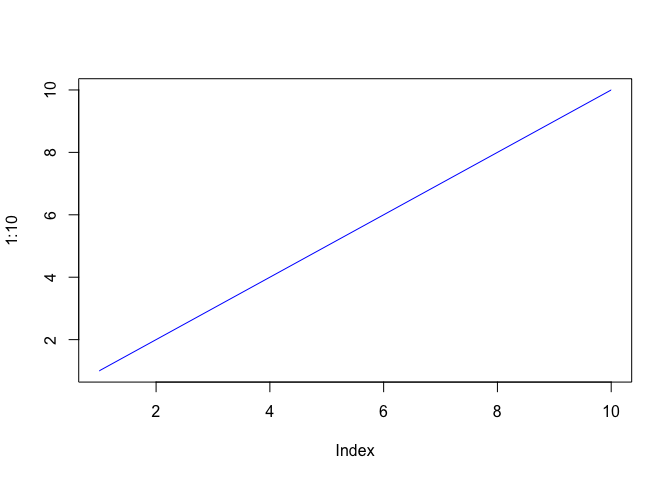
\includegraphics{Lec_05_Handout_files/figure-latex/unnamed-chunk-1-1.pdf}

\begin{Shaded}
\begin{Highlighting}[]
\NormalTok{weight}\OperatorTok{$}\NormalTok{Age}
\end{Highlighting}
\end{Shaded}

\begin{verbatim}
##  [1] 0 1 2 3 4 5 6 7 8 9
\end{verbatim}

\begin{Shaded}
\begin{Highlighting}[]
\NormalTok{weight}\OperatorTok{$}\NormalTok{Weight}
\end{Highlighting}
\end{Shaded}

\begin{verbatim}
##  [1] 3.6 4.4 5.2 6.0 6.6 7.2 7.8 8.4 8.8 9.2
\end{verbatim}

\begin{Shaded}
\begin{Highlighting}[]
\KeywordTok{plot}\NormalTok{(weight}\OperatorTok{$}\NormalTok{Age, weight}\OperatorTok{$}\NormalTok{Weight)}
\end{Highlighting}
\end{Shaded}

\includegraphics{Lec_05_Handout_files/figure-latex/unnamed-chunk-1-2.pdf}

\begin{Shaded}
\begin{Highlighting}[]
\CommentTok{# 2B: Barplot}
\CommentTok{# read in table}
\CommentTok{# use sep = "\textbackslash{}t" as argument for tab delimited data}
\NormalTok{nfeatures <-}\StringTok{ }\KeywordTok{read.table}\NormalTok{(}\StringTok{"bimm143_05_rstats/feature_counts.txt"}\NormalTok{, }
                        \DataTypeTok{sep =} \StringTok{"}\CharTok{\textbackslash{}t}\StringTok{"}\NormalTok{, }\DataTypeTok{header =} \OtherTok{TRUE}\NormalTok{)}
\CommentTok{# View table}
\CommentTok{#View(nfeatures)}
\CommentTok{# make default barplot}
\KeywordTok{barplot}\NormalTok{(nfeatures}\OperatorTok{$}\NormalTok{Count)}
\end{Highlighting}
\end{Shaded}

\includegraphics{Lec_05_Handout_files/figure-latex/unnamed-chunk-1-3.pdf}

\begin{Shaded}
\begin{Highlighting}[]
\CommentTok{# change global plot margin parameters}
\KeywordTok{par}\NormalTok{(}\DataTypeTok{mar =} \KeywordTok{c}\NormalTok{(}\FloatTok{5.1}\NormalTok{, }\FloatTok{10.1}\NormalTok{, }\FloatTok{4.1}\NormalTok{, }\FloatTok{4.1}\NormalTok{))}
\CommentTok{# make formatted barplot}
\KeywordTok{barplot}\NormalTok{(nfeatures}\OperatorTok{$}\NormalTok{Count, }
        \DataTypeTok{names.arg =}\NormalTok{ nfeatures}\OperatorTok{$}\NormalTok{Feature, }\CommentTok{# read in Feature vector as names}
        \DataTypeTok{horiz =} \OtherTok{TRUE}\NormalTok{, }\DataTypeTok{ylab =} \StringTok{""}\NormalTok{, }\DataTypeTok{xlab =} \StringTok{"Feature"}\NormalTok{, }\DataTypeTok{xlim =} \KeywordTok{c}\NormalTok{(}\DecValTok{0}\NormalTok{, }\DecValTok{80000}\NormalTok{),}
        \DataTypeTok{main =} \StringTok{"Feature Counts"}\NormalTok{, }\DataTypeTok{las =} \DecValTok{1}\NormalTok{, }\CommentTok{# las = 1 makes horizontal text labels}
        \DataTypeTok{col =} \KeywordTok{rainbow}\NormalTok{(}\DecValTok{12}\NormalTok{)) }\CommentTok{# use colors}
\end{Highlighting}
\end{Shaded}

\includegraphics{Lec_05_Handout_files/figure-latex/unnamed-chunk-1-4.pdf}

\begin{Shaded}
\begin{Highlighting}[]
\CommentTok{# 2C: Histograms}
\NormalTok{x <-}\StringTok{ }\KeywordTok{c}\NormalTok{(}\KeywordTok{rnorm}\NormalTok{(}\DecValTok{10000}\NormalTok{), }\KeywordTok{rnorm}\NormalTok{(}\DecValTok{10000}\NormalTok{) }\OperatorTok{+}\StringTok{ }\DecValTok{4}\NormalTok{) }\CommentTok{# generate distributions}
\KeywordTok{hist}\NormalTok{(x) }\CommentTok{# default}
\end{Highlighting}
\end{Shaded}

\includegraphics{Lec_05_Handout_files/figure-latex/unnamed-chunk-1-5.pdf}

\begin{Shaded}
\begin{Highlighting}[]
\KeywordTok{hist}\NormalTok{(x, }\DataTypeTok{breaks =} \DecValTok{100}\NormalTok{)}
\end{Highlighting}
\end{Shaded}

\includegraphics{Lec_05_Handout_files/figure-latex/unnamed-chunk-1-6.pdf}

\begin{Shaded}
\begin{Highlighting}[]
\CommentTok{# 3A: Providing Color Vectors}
\CommentTok{# read in table using read.delim (US)}
\NormalTok{counts <-}\StringTok{ }\KeywordTok{read.delim}\NormalTok{(}\StringTok{"bimm143_05_rstats/male_female_counts.txt"}\NormalTok{) }
\CommentTok{#read.delim2 uses comma instead of decimal}
\CommentTok{#View(counts)}
\KeywordTok{par}\NormalTok{(}\DataTypeTok{mar =} \KeywordTok{c}\NormalTok{(}\DecValTok{6}\NormalTok{, }\DecValTok{5}\NormalTok{, }\DecValTok{4}\NormalTok{, }\DecValTok{4}\NormalTok{))}

\CommentTok{# you can type multipe lines at once by holding down option + command}
\KeywordTok{barplot}\NormalTok{(counts}\OperatorTok{$}\NormalTok{Count,}
        \DataTypeTok{names.arg =}\NormalTok{ counts}\OperatorTok{$}\NormalTok{Sample,}
        \DataTypeTok{las =} \DecValTok{2}\NormalTok{,}
        \DataTypeTok{col =} \KeywordTok{c}\NormalTok{(}\StringTok{"red"}\NormalTok{, }\StringTok{"black"}\NormalTok{, }\StringTok{"white"}\NormalTok{),}
        \DataTypeTok{ylim =} \KeywordTok{c}\NormalTok{(}\DecValTok{0}\NormalTok{, }\DecValTok{20}\NormalTok{),}
        \DataTypeTok{ylab =} \StringTok{"Frequency"}\NormalTok{)}
\end{Highlighting}
\end{Shaded}

\includegraphics{Lec_05_Handout_files/figure-latex/unnamed-chunk-1-7.pdf}

\begin{Shaded}
\begin{Highlighting}[]
\CommentTok{# you can type multipe lines at once by holding down option + command}
\KeywordTok{barplot}\NormalTok{(counts}\OperatorTok{$}\NormalTok{Count,}
        \DataTypeTok{names.arg =}\NormalTok{ counts}\OperatorTok{$}\NormalTok{Sample,}
        \DataTypeTok{las =} \DecValTok{2}\NormalTok{,}
        \DataTypeTok{col =} \KeywordTok{heat.colors}\NormalTok{(}\DecValTok{0}\NormalTok{), }\CommentTok{# heat map colors}
        \DataTypeTok{ylim =} \KeywordTok{c}\NormalTok{(}\DecValTok{0}\NormalTok{, }\DecValTok{20}\NormalTok{),}
        \DataTypeTok{ylab =} \StringTok{"Frequency"}\NormalTok{)}
\end{Highlighting}
\end{Shaded}

\includegraphics{Lec_05_Handout_files/figure-latex/unnamed-chunk-1-8.pdf}


\end{document}
